\documentclass[t,usenames,dvipsnames]{beamer}
\usetheme{Copenhagen}
\setbeamertemplate{headline}{} % remove toc from headers
\beamertemplatenavigationsymbolsempty

\usepackage{amsmath, tcolorbox, bm, tikz, pgfplots}
\pgfplotsset{compat = 1.16}

\everymath{\displaystyle}

\title{Simplifying Radical Expressions}
\author{}
\date{}

\AtBeginSection[]
{
  \begin{frame}
    \frametitle{Objectives}
    \tableofcontents[currentsection]
  \end{frame}
}

\begin{document}

\begin{frame}
    \maketitle
\end{frame}

\section{Write radicals as rational exponents and vice versa.}

\begin{frame}{Radicand}
\begin{tcolorbox}[colframe=green!20!black, colback = green!30!white,title=\textbf{Radicand}]
For $\sqrt[n]{a}$, the \textbf{radicand} is $\bm{a}$.
\end{tcolorbox}
\end{frame}

\begin{frame}{Radicals}
What is $\left(\sqrt[3]{27}\right)^2$? \newline\\

Well, if we evaluate $\sqrt[3]{27}$ first, we get 3. Then when we square that, we get the final answer of 9. 
\end{frame}

\begin{frame}{Radicals} 
To put things visually, suppose the block below represents 27.  

\begin{center}
    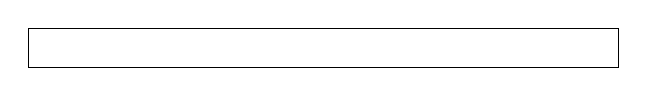
\begin{tikzpicture}[scale=0.5]
    \draw (0,0) rectangle (15,1);
    \end{tikzpicture}
\end{center}

Since we are taking the cube root, we can divide the large block up into 3 equal blocks where we multiply by 3 to get each new number. (\emph{Note}: We can divide it up into 2 equal blocks for square root, 3 for cube root, 4 for fourth root, etc.):
\begin{center}
    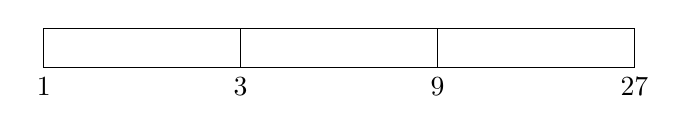
\begin{tikzpicture}[scale=0.5]
    \draw (0,0) rectangle (15,1);
    \node at (0,0) [anchor=north] {1};
    \node at (15,0) [anchor=north] {27};
    \draw (5,0) -- (5,1);
    \node at (5,0) [anchor=north] {3};
    \draw (10,0) -- (10,1);
    \node at (10,0) [anchor=north] {9};
    \end{tikzpicture}
\end{center}
\end{frame}

\begin{frame}{Radicals}
Now let's look what happens as we shade in the block from the left, up to our answer of 9:
\begin{center}
    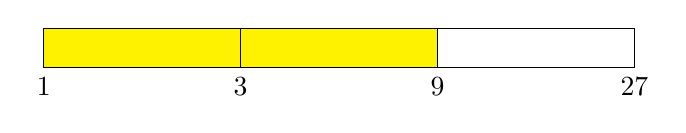
\begin{tikzpicture}[scale=0.5]
    \draw (0,0) [fill=yellow, color=yellow] rectangle (5,1);
    \draw (5,0) [fill=yellow, color=yellow] rectangle (10,1);
    \draw (0,0) rectangle (15,1);
    \node at (0,0) [anchor=north] {1};
    \node at (15,0) [anchor=north] {27};
    \draw (5,0) -- (5,1);
    \node at (5,0) [anchor=north] {3};
    \draw (10,0) -- (10,1);
    \node at (10,0) [anchor=north] {9};
    \end{tikzpicture}
\end{center}

Notice that out of the three equal areas, two of them are shaded. \newline\\

This is a visual approach to the idea that $\left(\sqrt[3]{27}\right)^2 = 27^{2/3}$   \newline\\

In general,
\[
\sqrt[\text{root}]{x^{\text{power}}} = x^{\text{power/root}}
\]
\end{frame}

\begin{frame}{Example 1}
Write each of the following using rational exponents.	\newline\\
(a) \quad $\sqrt{6}$		\pause	\vspace{6pt}
\[ 6^{1/2} \]	\pause	\vspace{6pt}
(b) \quad $\sqrt[3]{8}$	\pause	\vspace{6pt}
\[ 8^{1/3} \] \pause	\vspace{6pt}
(c) \quad $\sqrt[4]{x^3}$	\pause	\vspace{6pt}
\[ x^{3/4} \]
\end{frame}

\begin{frame}{Example 2}
Write each of the following in radical form.	\newline\\
(a)	\quad	$5^{1/2}$	\pause \vspace{6pt}
\[ \sqrt{5} \]	\pause \vspace{6pt}
(b)	\quad	$(-9)^{5/3}$	\pause \vspace{6pt}
\[	\sqrt[3]{(-9)^5} \] \pause \vspace{6pt}
(c)	\quad	$x^{-1/3}$	\pause \vspace{6pt}
\[ \sqrt[3]{x^{-1}} \text{\quad or \quad} \sqrt[3]{\frac{1}{x}} \]	
\end{frame}

\section{Simplify square root and higher root expressions.}

\begin{frame}{Even Roots and Exponents}
When dealing with \textbf{even} roots and exponents, keep in mind that the root and exponent don't ``cancel each other out."
\newline\\


For instance, $\sqrt{5^2}=\sqrt{25}=5$, but $\sqrt{(-5)^2}=\sqrt{25}=5$.
\end{frame}

\begin{frame}{Even Roots and Exponents}
The graphs of $y = \sqrt{x^2}$ and $y=|x|$ are shown. Notice they are identical.
\newline\\

\begin{tabular}{cc}
    {\color{blue}$y = \sqrt{x^2}$}    &   {\color{red}$y = |x|$}   \\[11pt]
    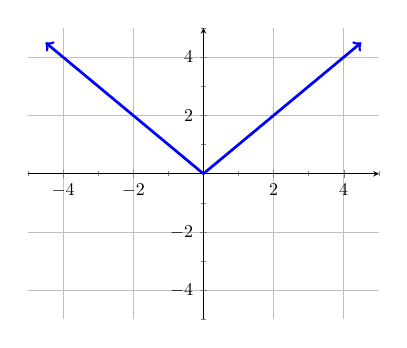
\begin{tikzpicture}[scale=0.65]
    \begin{axis}
    [
        xmin = -5,
        xmax = 5,
        ymin = -5,
        ymax = 5,
        axis lines = middle,
        grid,
        minor tick num = 1
    ]
    \addplot [<->, color = blue, line width = 1.5, domain=-4.5:4.5, samples = 300] {abs(x)};
    \end{axis}
    \end{tikzpicture}
    &
    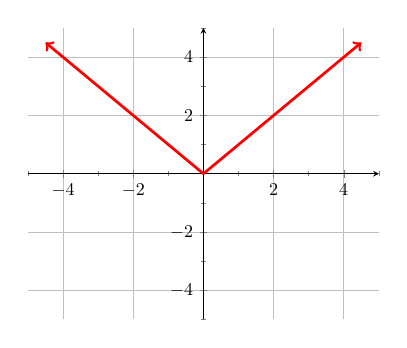
\begin{tikzpicture}[scale=0.65]
    \begin{axis}
    [
        xmin = -5,
        xmax = 5,
        ymin = -5,
        ymax = 5,
        axis lines = middle,
        grid,
        minor tick num = 1
    ]
    \addplot [<->, color = red, line width = 1.5, domain=-4.5:4.5, samples = 300] {abs(x)};
    \end{axis}
    \end{tikzpicture}
\end{tabular}
\vspace{8pt}

Thus, for any real number $x$, $\sqrt{x^2} = |x|$.
\end{frame}

\begin{frame}{Odd Roots and Exponents}
Odd roots, such as $\sqrt[3]{\quad}$ do not follow the same rule as even roots.
\newline\\

So for any real number $x$, $\sqrt[3]{x^3} = x$.
\newline\\

And, in general, for any real number $x$,	\newline\\
\begin{enumerate}
	\item If $n$ is even, $\sqrt[n]{x^n} = |x|$.	\newline\\
	\item If $n$ is odd, $\sqrt[n]{x^n} = x$.
\end{enumerate}
\end{frame}

\begin{frame}{Example 3}
Simplify each of the following. Exact answers only. Use absolute value bars when necessary.		\newline\\
(a) \quad $\sqrt{72x^2}$
\begin{align*}
\onslide<2->{\sqrt{72x^2} &= \sqrt{72} \cdot \sqrt{x^2}} \\[8pt]
\onslide<3->{&= 6\sqrt{2} \cdot |x|} \\[8pt]
\onslide<4->{&= 6|x| \sqrt{2}}
\end{align*}
\end{frame}

\begin{frame}{Example 3}
(b) \quad $\sqrt{175x^3}$
\begin{align*}
\onslide<2->{\sqrt{175x^3} &= \sqrt{175} \cdot \sqrt{x^3}} \\[8pt]
\onslide<3->{&= 5\sqrt{7} \cdot |x|\sqrt{x}} \\[8pt]
\onslide<4->{&= 5|x|\sqrt{7x}}
\end{align*}
\end{frame}

\begin{frame}{Example 3}
(c) \quad $\sqrt{18x^4}$
\begin{align*}
\onslide<2->{\sqrt{18x^4} &= \sqrt{18} \cdot \sqrt{x^4}} \\[8pt]
\onslide<3->{&= 3\sqrt{2} \cdot x^2} \\[8pt]
\onslide<4->{&= 3x^2\cdot \sqrt{2}}
\end{align*}
\end{frame}

\begin{frame}{Example 3}
(d) \quad $\sqrt{65x^5}$
\begin{align*}
\onslide<2->{\sqrt{65x^5} &= \sqrt{65} \cdot \sqrt{x^5}} \\[8pt]
\onslide<3->{&= \sqrt{65} \cdot x^2\sqrt{x}} \\[8pt]
\onslide<4->{&= x^2\cdot \sqrt{65x}}
\end{align*}
\end{frame}

\begin{frame}{Example 3}
(e) \quad $\sqrt[3]{27x^7}$
\begin{align*}
\onslide<2->{\sqrt[3]{27x^7} &= \sqrt[3]{27} \cdot \sqrt[3]{x^7}} \\[8pt]
\onslide<3->{&= 3 \cdot x^2\sqrt[3]{x}} \\[8pt]
\onslide<4->{&= 3x^2\cdot \sqrt[3]{x}}
\end{align*}
\end{frame}

\begin{frame}{Example 3}
(f) \quad $\sqrt[3]{128x^6}$
\begin{align*}
\onslide<2->{\sqrt[3]{128x^6} &= \sqrt[3]{128} \cdot \sqrt[3]{x^6}} \\[8pt]
\onslide<3->{&= 4\cdot\sqrt[3]{2} \cdot x^2} \\[8pt]
\onslide<4->{&= 4x^2\cdot \sqrt[3]{2}}
\end{align*}
\end{frame}

\section{Perform operations with radical expressions.}

\begin{frame}{Performing Operations with Radical Expressions}
Once we have simplified the radicals, we can add and subtract radical expressions with the same radicands and roots. This is essentially combining like terms.
\end{frame}

\begin{frame}{Example 4}
Simplify each of the following. Exact answers only.	\newline\\
(a)	\quad	$\sqrt{98} + \sqrt{8}$
\begin{align*}
\onslide<2->{\sqrt{98} + \sqrt{8} &= 7\sqrt{2} + 2\sqrt{2}} \\[8pt]
\onslide<3->{&= 9\sqrt{2}}
\end{align*}
\end{frame}

\begin{frame}{Example 4}
(b)	\quad	$\sqrt{108x} - \sqrt{300x}$
\begin{align*}
\onslide<2->{\sqrt{108x} - \sqrt{300x} &= 6\sqrt{3x} - 10\sqrt{3x}} \\[8pt]
\onslide<3->{&= -4\sqrt{3x}}
\end{align*}
\end{frame}

\begin{frame}{Example 4}
(c)	\quad	$4\sqrt{6} + 3\sqrt{54} - 5\sqrt{45}$
\begin{align*}
\onslide<2->{4\sqrt{6} + 3\sqrt{54} - 5\sqrt{45} &= 4\sqrt{6} + 3(3\sqrt{6}) - 5(3\sqrt{5})} \\[8pt]
\onslide<3->{&= 4\sqrt{6} + 9\sqrt{6} - 15\sqrt{5}} \\[8pt]
\onslide<4->{&= 13\sqrt{6} - 15\sqrt{5}}
\end{align*}
\end{frame}

\begin{frame}{Multiplying and Dividing Radical Expressions}
We can also multiply and divide radical expressions. It may be helpful to convert them to rational exponent form first, and then use your laws of exponents.
\end{frame}

\begin{frame}{Example 5}
Simplify each of the following. Leave no radical expressions in a denominator.	\newline\\
(a)	\quad $\sqrt{x^5} \cdot \sqrt{x^2}$
\begin{align*}
\onslide<2->{\sqrt{x^5} \cdot \sqrt{x^2} &= x^{5/2} \cdot x^{2/2}} \\[8pt]
\onslide<3->{&= x^{7/2}} \\[8pt]
\onslide<4->{&= \sqrt{x^7}} \\[8pt]
\onslide<5->{&= |x^3|\sqrt{x}}
\end{align*}
\end{frame}

\begin{frame}{Example 5}
(b)	\quad $\sqrt{a^3} \cdot \sqrt[3]{a^2}$
\begin{align*}
\onslide<2->{\sqrt{a^3} \cdot \sqrt[3]{a^2} &= a^{3/2} \cdot a^{2/3}} \\[8pt]
\onslide<3->{&= a^{13/6}} \\[8pt]
\onslide<4->{&= \sqrt[6]{a^{13}}} \\[8pt]
\onslide<5->{&= a^2 \cdot \sqrt[6]{a}}
\end{align*}
\end{frame}

\begin{frame}{Example 5}
(c)	\quad $\sqrt[3]{y^6} \cdot \sqrt{y^3}$
\begin{align*}
\onslide<2->{\sqrt[3]{y^6} \cdot \sqrt{y^3} &= y^{6/3} \cdot y^{3/2}} \\[8pt]
\onslide<3->{&= y^{7/2}} \\[8pt]
\onslide<4->{&= \sqrt{y^7}} \\[8pt]
\onslide<5->{&= |y^3| \cdot \sqrt{y}}
\end{align*}
\end{frame}

\begin{frame}{Example 5}
(d)	\quad $\dfrac{\sqrt{x^5}}{\sqrt{x}}$
\begin{align*}
\onslide<2->{\frac{\sqrt{x^5}}{\sqrt{x}} &= \frac{x^{5/2}}{x^{1/2}}} \\[12pt]
\onslide<3->{&= x^{4/2}} \\[12pt]
\onslide<4->{&= x^2}
\end{align*}
\end{frame}

\begin{frame}{Example 5}
(e)	\quad $\dfrac{7}{\sqrt{2}}$
\begin{align*}
\onslide<2->{\frac{7}{\sqrt{2}}&=\frac{7}{2^{1/2}}} \\[12pt]
\onslide<3->{&= \frac{7}{2^{1/2}} \left(\frac{2^{1/2}}{2^{1/2}} \right)} \\[12pt]
\onslide<4->{&= \frac{7\cdot 2^{1/2}}{2}} \\[12pt]
\onslide<5->{&= \frac{7\sqrt{2}}{2}}
\end{align*}
\end{frame}

\begin{frame}{Example 5}
(f) \quad $\dfrac{\sqrt[3]{y^6}}{\sqrt{y^3}}$
\begin{align*}
\onslide<2->{\frac{\sqrt[3]{y^6}}{\sqrt{y^3}} &= \frac{y^{6/3}}{y^{3/2}}}	\\[12pt]
\onslide<3->{&= y^{1/2}} \\[12pt]
\onslide<4->{&= \sqrt{y}}
\end{align*}
\end{frame}

\end{document}
